%%%%%%%%%%%%%%%%%%%%%%%%%%%%%%%%%%%%%%%%%%%%%%%%%%%%%%%%%%%%%%%%%%%%%%%%%%%%%%%
%% SOCIOL 723 -- Social Statistics II
%% Math Review: Calculus, Taylor Expansion, Linear Algebra, Probability,
%%              and Asymptotics, as This Course Uses Them
%% Wenhao Jiang, Duke University, Fall 2026
%%%%%%%%%%%%%%%%%%%%%%%%%%%%%%%%%%%%%%%%%%%%%%%%%%%%%%%%%%%%%%%%%%%%%%%%%%%%%%%
\documentclass[11pt]{article}

\usepackage[T1]{fontenc}
\usepackage{lmodern}
\usepackage[margin=1.1in]{geometry}
\usepackage{amsmath,amsfonts,amssymb,bm}
\usepackage{amsthm}
\usepackage{booktabs}
\usepackage{microtype}
\usepackage{enumitem}
\usepackage{tikz}
\usetikzlibrary{arrows.meta,calc}
\usepackage[dvipsnames]{xcolor}
\usepackage[most]{tcolorbox}
\usepackage{titlesec}
\usepackage{fancyhdr}
\usepackage{setspace}
\usepackage[colorlinks=true,linkcolor=dukeblue,citecolor=dukeblue,urlcolor=dukeblue]{hyperref}
\setstretch{1.12}
\setlist{itemsep=2pt,topsep=3pt}

\definecolor{dukeblue}{RGB}{1,33,105}
\definecolor{accent}{RGB}{200,78,0}
\definecolor{softgray}{RGB}{244,244,247}
\definecolor{softblue}{RGB}{236,240,249}
\definecolor{softorange}{RGB}{252,243,236}

%% ---- headings ---------------------------------------------------------------
\titleformat{\section}{\Large\bfseries\color{dukeblue}}{\thesection}{0.7em}{}
\titleformat{\subsection}{\large\bfseries\color{dukeblue}}{\thesubsection}{0.6em}{}
\titlespacing*{\section}{0pt}{18pt}{8pt}
\titlespacing*{\subsection}{0pt}{12pt}{5pt}

%% ---- running head ----------------------------------------------------------
\pagestyle{fancy}
\fancyhf{}
\fancyhead[L]{\small\color{gray}SOCIOL 723 \ $\cdot$\ Math Review}
\fancyhead[R]{\small\color{gray}\nouppercase{\leftmark}}
\fancyfoot[C]{\small\thepage}
\renewcommand{\headrulewidth}{0.3pt}
\renewcommand{\headrule}{\hbox to\headwidth{\color{gray!60}\leaders\hrule height \headrulewidth\hfill}}

%% ---- boxes -----------------------------------------------------------------
\newtcolorbox{rulebox}[1][]{enhanced,breakable,colback=softblue,colframe=dukeblue,
  boxrule=0.6pt,arc=2pt,left=8pt,right=8pt,top=5pt,bottom=5pt,
  fonttitle=\bfseries,coltitle=white,colbacktitle=dukeblue,
  title={Rule\ifx\relax#1\relax\else: #1\fi},attach boxed title to top left={yshift=-2mm,xshift=4mm},
  boxed title style={arc=1pt,boxrule=0pt}}
\newtcolorbox{takeaway}{enhanced,breakable,colback=softorange,colframe=accent,
  boxrule=0.6pt,arc=2pt,left=8pt,right=8pt,top=5pt,bottom=5pt,
  fonttitle=\bfseries,coltitle=white,colbacktitle=accent,
  title={What to keep},attach boxed title to top left={yshift=-2mm,xshift=4mm},
  boxed title style={arc=1pt,boxrule=0pt}}
\newtcolorbox{inthecourse}{enhanced,breakable,colback=softgray,colframe=gray!70,
  boxrule=0.4pt,arc=2pt,left=8pt,right=8pt,top=4pt,bottom=4pt,
  fonttitle=\bfseries\small,coltitle=black!70,
  title={Where this appears in the course},detach title,before upper={\tcbtitle\par\smallskip}}

\theoremstyle{definition}
\newtheorem{example}{Example}[section]
\newtheorem{exercise}{Exercise}

\DeclareMathOperator{\Var}{Var}
\DeclareMathOperator{\Cov}{Cov}
\DeclareMathOperator{\rank}{rank}
\DeclareMathOperator*{\argmin}{arg\,min}
\DeclareMathOperator{\plim}{plim}
\newcommand{\E}{E}
\newcommand{\R}{\mathbb{R}}
\newcommand{\loglik}{\ell}
\newcommand{\Info}{\mathcal{I}}
\newcommand{\X}{\bm{X}}
\newcommand{\Y}{\bm{y}}
\newcommand{\bbeta}{\bm{\beta}}
\newcommand{\bhat}{\hat{\bm{\beta}}}
\newcommand{\dd}{\mathrm{d}}
\newcommand{\ind}{\mathbb{1}}
\newcommand{\dto}{\overset{d}{\longrightarrow}}
\newcommand{\pto}{\overset{p}{\longrightarrow}}

\begin{document}

%% ---- title -----------------------------------------------------------------
\thispagestyle{empty}
\begin{center}
{\color{dukeblue}\rule{\linewidth}{1.2pt}}\\[14pt]
{\LARGE\bfseries\color{dukeblue} Math Review}\\[8pt]
{\large Calculus, Taylor Expansion, Linear Algebra, Probability, and
Asymptotics,\\ as This Course Uses Them}\\[14pt]
{\normalsize Wenhao Jiang \ $\cdot$\ SOCIOL 723, Social Statistics II
\ $\cdot$\ Duke University \ $\cdot$\ Fall 2026}\\[10pt]
{\color{dukeblue}\rule{\linewidth}{1.2pt}}
\end{center}
\vskip 14pt

\section*{How to read this}

This is not a mathematics course. It is the smallest set of tools that the
lectures lean on, written slowly, with every rule followed by the place in
the course where you will meet it. Nothing here is examined for its own
sake; all of it is examined through the statistics.

\begin{center}\small
\renewcommand{\arraystretch}{1.25}
\begin{tabular}{p{0.34\linewidth}p{0.44\linewidth}c}
\toprule
Tool & Where it appears & Section \\
\midrule
derivative, chain rule, $\log$ and $\exp$ & score function, log-likelihood (W3) & \ref{sec:deriv} \\
second derivative, concavity & information, standard errors (W3) & \ref{sec:second} \\
first- and second-order conditions & the MLE, OLS (W1, W3) & \ref{sec:max} \\
partial derivatives, gradient, Hessian & several parameters at once (W3, W4) & \ref{sec:partial} \\
Taylor expansion & Wald versus LR, Newton, delta method (W3, W4, W14) & \ref{sec:taylor} \\
vectors, matrices, transpose, inverse & $X'\beta$, $(X'X)^{-1}X'y$, FWL (W1, W10, W13) & \ref{sec:linalg} \\
quadratic forms, matrix derivatives & OLS and ridge in matrix form, variance matrices (W1, W2, W12) & \ref{sec:matcalc} \\
expectation, variance, covariance & causal estimands, IV, weighting (W5, W6, W7) & \ref{sec:prob} \\
conditional expectation, iterated expectations, Bayes & CEF, propensity scores, matching (W1, W5, W6) & \ref{sec:condexp} \\
limits, LLN, CLT, plims & consistency, asymptotic normality, sandwich (W2, W3, W7) & \ref{sec:asymp} \\
integrals, kernels & survival and hazard (W4), local regression (W9) & \ref{sec:integrals} \\
constrained and penalized optimization & synthetic control (W11), ridge and lasso (W12), orthogonality (W13) & \ref{sec:constrained} \\
\bottomrule
\end{tabular}
\end{center}

If calculus is years away, read Sections~\ref{sec:functions}
to~\ref{sec:taylor} in order, doing the exercises. If calculus is fresh but
matrices are not, start at Section~\ref{sec:linalg}. Sections~\ref{sec:prob}
to~\ref{sec:constrained} are what the causal-inference and machine-learning
weeks need; read them before Week 5. Answers to all exercises are at the end.

%%%%%%%%%%%%%%%%%%%%%%%%%%%%%%%%%%%%%%%%%%%%%%%%%%%%%%%%%%%%%%%%%%%%%%%%%%%%%%%
\section{Functions, sums, logs, and exponentials}
\label{sec:functions}

\subsection{Functions and the notation we use}

A function takes a number in and gives a number out: $f(x) = x^2$ takes $3$
to $9$. In statistics the input is usually a \emph{parameter} we are free to
choose, and the output is how well that parameter explains the data. Week 3's
central object is exactly such a function: the log-likelihood
$\loglik(\theta)$, where $\theta$ is a candidate value of the parameter and
$\loglik(\theta)$ is a score for it. Much of the course is about finding
where such functions peak and how sharply.

Two pieces of notation appear on every page.
\begin{itemize}
  \item \textbf{Sums.} $\sum_{i=1}^{n} x_i$ means $x_1 + x_2 + \cdots + x_n$.
        The index $i$ runs over observations. A constant comes out of a sum,
        $\sum_i c\,x_i = c \sum_i x_i$, and a sum of a constant is $n$ times
        it, $\sum_{i=1}^n c = nc$. The sample mean is $\bar x =
        \frac1n\sum_i x_i$.
  \item \textbf{Products.} $\prod_{i=1}^{n} x_i$ means $x_1 x_2 \cdots x_n$.
        A likelihood is a product over observations, because independent
        observations multiply their probabilities.
\end{itemize}

\subsection{Exponentials and logarithms}

The number $e \approx 2.718$ is the base of the natural exponential $e^x$,
also written $\exp(x)$. Its inverse is the natural logarithm $\log x$ (in
this course $\log$ always means natural log; some books write $\ln$). So
$\log(e^x) = x$ and $e^{\log x} = x$. The log is defined only for $x > 0$;
$e^x$ is defined for every $x$ and is always positive.

\begin{rulebox}[exponents]
$e^{a}e^{b} = e^{a+b}$, \quad $(e^{a})^{b} = e^{ab}$, \quad $e^{-a} = 1/e^{a}$,
\quad $e^0 = 1$.
\end{rulebox}

\begin{rulebox}[logs]
$\log(ab) = \log a + \log b$, \quad $\log(a/b) = \log a - \log b$, \quad
$\log(a^{b}) = b\log a$, \quad $\log 1 = 0$.
\end{rulebox}

The first log rule is the reason the course works with log-likelihoods at
all. A likelihood is a product of $n$ probabilities; its log is a sum of
$n$ logs:
\begin{align*}
  \log \prod_{i=1}^{n} f(y_i \mid \theta) = \sum_{i=1}^{n} \log f(y_i \mid \theta) .
\end{align*}
Sums are easier to differentiate than products, and a product of 500
numbers below one underflows to zero on a computer while its log is a
perfectly ordinary negative number (Lab 3 shows this).

\begin{example}[Bernoulli log-likelihood, Week 3]
Each $y_i$ is $1$ with probability $\theta$ and $0$ with probability
$1-\theta$, so $f(y_i \mid \theta) = \theta^{y_i}(1-\theta)^{1-y_i}$. Then
\begin{align*}
  \loglik(\theta) = \sum_{i=1}^{n}\log\big[\theta^{y_i}(1-\theta)^{1-y_i}\big]
  = \sum_{i=1}^{n}\big[y_i\log\theta + (1-y_i)\log(1-\theta)\big]
  = s\log\theta + (n-s)\log(1-\theta),
\end{align*}
where $s = \sum_i y_i$ is the number of ones. The second equality used
$\log(ab) = \log a + \log b$ and $\log a^b = b\log a$; the third used that
$\log\theta$ does not depend on $i$, so it comes out of the sum.
\end{example}

\subsection{The logistic function}

One function recurs from Week 4 on: the logistic function
\begin{align*}
  \Lambda(z) = \frac{e^{z}}{1+e^{z}} = \frac{1}{1+e^{-z}} .
\end{align*}
It takes any real number $z$ to a number strictly between $0$ and $1$, which
is why it is used to turn a line $X'\beta$ into a probability. Two
identities you will use:
\begin{align*}
  1 - \Lambda(z) = \frac{1}{1+e^{z}},
  \qquad\qquad
  \log\frac{\Lambda(z)}{1-\Lambda(z)} = z .
\end{align*}
The second says that the logistic function is the inverse of the log-odds:
if $p = \Lambda(z)$ then $z = \log[p/(1-p)]$.

\begin{exercise}
Show the first identity: compute $1 - e^{z}/(1+e^{z})$ by putting both
terms over the common denominator $1+e^{z}$.
\end{exercise}

%%%%%%%%%%%%%%%%%%%%%%%%%%%%%%%%%%%%%%%%%%%%%%%%%%%%%%%%%%%%%%%%%%%%%%%%%%%%%%%
\section{Derivatives}
\label{sec:deriv}

\subsection{What a derivative is}

The derivative of $f$ at a point $x$ is the slope of $f$ there: how much
$f$ rises per unit step to the right, for a very small step. Formally,
\begin{align*}
  f'(x) = \lim_{h \to 0}\frac{f(x+h) - f(x)}{h},
\end{align*}
the rise over the run, with the run shrunk to nothing. Other notations for
the same thing: $\dfrac{\dd f}{\dd x}$, $\dfrac{\dd}{\dd x}f(x)$, and in the
lecture slides $S(\theta)$ for the derivative of the log-likelihood, called
the \emph{score}.

\begin{center}
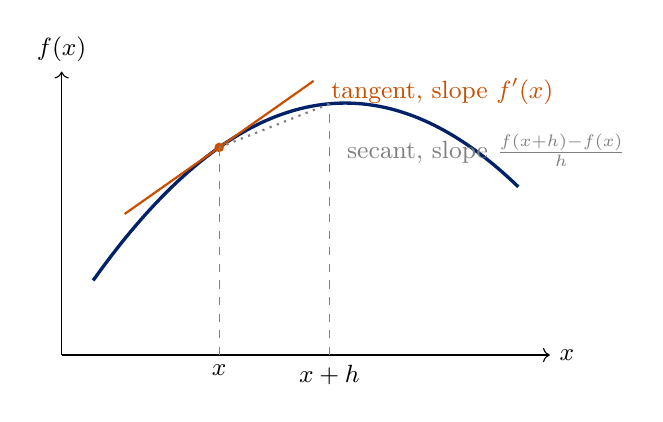
\begin{tikzpicture}[scale=1.0]
  \draw[->] (0,0) -- (6.2,0) node[right]{\small $x$};
  \draw[->] (0,0) -- (0,3.6) node[above]{\small $f(x)$};
  \draw[dukeblue,very thick,smooth,samples=80,domain=0.4:5.8,variable=\x]
    plot ({\x},{3.2-0.22*(\x-3.6)^2});
  \draw[accent,thick] (0.8,{2.6368-1.2*0.704}) -- (3.2,{2.6368+1.2*0.704});
  \fill[accent] (2,2.6368) circle (0.06);
  \draw[dashed,gray] (2,0) -- (2,2.6368);
  \node[below] at (2,0) {\small $x$};
  \node[accent,anchor=west] at (3.3,3.35) {\small tangent, slope $f'(x)$};
  \draw[gray,thick,dotted] (2,2.6368) -- (3.4,{3.2-0.22*(3.4-3.6)^2});
  \draw[dashed,gray] (3.4,0) -- (3.4,{3.2-0.22*(3.4-3.6)^2});
  \node[below] at (3.4,0) {\small $x+h$};
  \node[gray,anchor=west] at (3.5,2.6) {\small secant, slope $\frac{f(x+h)-f(x)}{h}$};
\end{tikzpicture}
\end{center}

The dotted line through two points on the curve has slope
$[f(x+h) - f(x)]/h$. As $h$ shrinks, the second point slides toward the
first and the dotted line turns into the tangent line at $x$. The
derivative is the slope of that tangent.

Three facts to hold on to:
\begin{itemize}
  \item $f'(x) > 0$ means $f$ is rising at $x$; $f'(x) < 0$ means falling.
  \item $f'(x) = 0$ means the tangent is flat: a peak, a trough, or a
        momentary plateau.
  \item The derivative is itself a function of $x$: the slope changes as
        you move along the curve. In the picture the slope is positive on
        the left, zero at the peak, negative on the right.
\end{itemize}

\subsection{The rules}

You never compute the limit directly. A handful of rules cover everything
in the course.

\begin{rulebox}[constants, powers, sums]
\begin{align*}
  \frac{\dd}{\dd x}\, c = 0, \qquad
  \frac{\dd}{\dd x}\, x^{k} = k\,x^{k-1}, \qquad
  \frac{\dd}{\dd x}\big[a f(x) + b g(x)\big] = a f'(x) + b g'(x).
\end{align*}
\end{rulebox}

The power rule with $k = 1$ gives $\frac{\dd}{\dd x}x = 1$; with $k = 2$,
$\frac{\dd}{\dd x}x^2 = 2x$; with $k = -1$, $\frac{\dd}{\dd x}\frac1x =
-\frac{1}{x^2}$. The third rule says a derivative goes through sums and
constant multiples term by term, so the derivative of a sum over
observations is the sum of the derivatives:
$\frac{\dd}{\dd\theta}\sum_i g_i(\theta) = \sum_i g_i'(\theta)$.

\begin{rulebox}[exponential and log]
\begin{align*}
  \frac{\dd}{\dd x}\, e^{x} = e^{x}, \qquad
  \frac{\dd}{\dd x}\, \log x = \frac{1}{x} .
\end{align*}
\end{rulebox}

The exponential is its own derivative, which is what makes it the natural
base. The log's derivative is $1/x$: it rises steeply near $0$ and ever
more slowly for large $x$.

\begin{rulebox}[product and quotient]
\begin{align*}
  \frac{\dd}{\dd x}\big[f(x)\,g(x)\big] = f'(x)\,g(x) + f(x)\,g'(x),
  \qquad
  \frac{\dd}{\dd x}\frac{f(x)}{g(x)} = \frac{f'(x)\,g(x) - f(x)\,g'(x)}{g(x)^2}.
\end{align*}
\end{rulebox}

\begin{rulebox}[chain rule]
If $y = f(u)$ and $u = g(x)$, so that $y = f(g(x))$, then
\begin{align*}
  \frac{\dd y}{\dd x} = f'(u)\cdot g'(x) = f'\big(g(x)\big)\cdot g'(x).
\end{align*}
\end{rulebox}

The chain rule is the one to internalize. Read it as: differentiate the
outer function, leaving the inside alone, then multiply by the derivative
of the inside. Two special cases do most of the work in this course:
\begin{align*}
  \frac{\dd}{\dd x}\log g(x) = \frac{g'(x)}{g(x)},
  \qquad\qquad
  \frac{\dd}{\dd x}e^{g(x)} = e^{g(x)}\, g'(x).
\end{align*}

\begin{example}[Each rule once]
\begin{align*}
  \frac{\dd}{\dd\theta}\log(1-\theta) &= \frac{-1}{1-\theta}
    && \text{chain rule: outer $\log$, inner $1-\theta$ with derivative $-1$} \\
  \frac{\dd}{\dd\theta}\big[s\log\theta\big] &= \frac{s}{\theta}
    && \text{constant times $\log$} \\
  \frac{\dd}{\dd x}\, e^{\beta_0 + \beta_1 x} &= \beta_1\, e^{\beta_0 + \beta_1 x}
    && \text{chain rule: outer $\exp$, inner derivative $\beta_1$} \\
  \frac{\dd}{\dd x}\,(y - a - bx)^2 &= 2(y - a - bx)\cdot(-b)
    && \text{chain rule: outer square, inner derivative $-b$} \\
  \frac{\dd}{\dd\theta}\, \theta e^{-\theta} &= e^{-\theta} - \theta e^{-\theta}
    && \text{product rule}
\end{align*}
\end{example}

\begin{example}[The score of the Bernoulli log-likelihood]
From Section~\ref{sec:functions},
$\loglik(\theta) = s\log\theta + (n-s)\log(1-\theta)$. Differentiate term
by term:
\begin{align*}
  S(\theta) = \loglik'(\theta) = \frac{s}{\theta} - \frac{n-s}{1-\theta}.
\end{align*}
The minus sign in the second term is the chain rule acting on $1-\theta$.
This is the ``Bernoulli: Deriving $\hat\theta$'' slide of Week 3.
\end{example}

\begin{example}[The derivative of the logistic function]
\label{ex:logistic-deriv}
Write $\Lambda(z) = (1+e^{-z})^{-1}$ and use the chain rule twice (outer
power $-1$, inner $1+e^{-z}$, whose derivative is $-e^{-z}$):
\begin{align*}
  \Lambda'(z) = -(1+e^{-z})^{-2}\cdot(-e^{-z}) = \frac{e^{-z}}{(1+e^{-z})^{2}}
  = \frac{1}{1+e^{-z}}\cdot\frac{e^{-z}}{1+e^{-z}} = \Lambda(z)\,\big(1-\Lambda(z)\big).
\end{align*}
The last step uses $e^{-z}/(1+e^{-z}) = 1/(1+e^{z}) = 1 - \Lambda(z)$.
This identity is the whole engine of the logit score in Week 4: the slope of
the logistic curve at $z$ is $p(1-p)$, largest at $p = 0.5$ and near zero
in the tails.
\end{example}

\begin{exercise}
Differentiate with respect to $\theta$: (a) $10\log\theta - 5\theta$;
(b) $\log(1+e^{\theta})$; (c) $-\tfrac{1}{2\sigma^2}(y - \theta)^2$.
\end{exercise}

\subsection{Second derivatives and curvature}
\label{sec:second}

The derivative of the derivative, $f''(x)$, says how the slope is changing.
\begin{itemize}
  \item $f''(x) < 0$: the slope is decreasing as you move right; the curve
        bends downward, like a hill. Such a function is \textbf{concave}
        there.
  \item $f''(x) > 0$: the slope is increasing; the curve bends upward, like
        a bowl. \textbf{Convex}.
  \item $|f''(x)|$ large: the curve bends sharply. Small: nearly a straight
        line.
\end{itemize}

\begin{center}
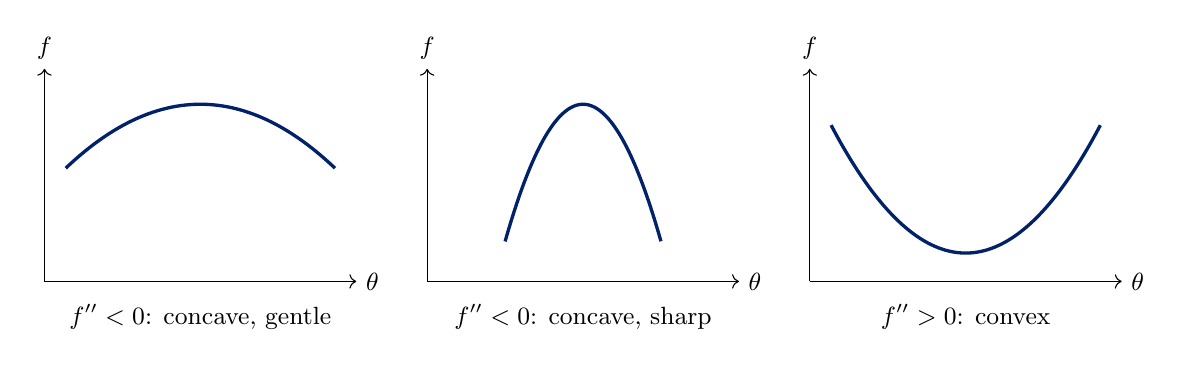
\begin{tikzpicture}[scale=0.9]
  \begin{scope}
    \draw[->] (0,0) -- (4.4,0) node[right]{\small $\theta$};
    \draw[->] (0,0) -- (0,3) node[above]{\small $f$};
    \draw[dukeblue,very thick,smooth,samples=60,domain=0.3:4.1,variable=\x]
      plot ({\x},{2.5-0.25*(\x-2.2)^2});
    \node at (2.2,-0.5) {\small $f'' < 0$: concave, gentle};
  \end{scope}
  \begin{scope}[xshift=5.4cm]
    \draw[->] (0,0) -- (4.4,0) node[right]{\small $\theta$};
    \draw[->] (0,0) -- (0,3) node[above]{\small $f$};
    \draw[dukeblue,very thick,smooth,samples=60,domain=1.1:3.3,variable=\x]
      plot ({\x},{2.5-1.6*(\x-2.2)^2});
    \node at (2.2,-0.5) {\small $f'' < 0$: concave, sharp};
  \end{scope}
  \begin{scope}[xshift=10.8cm]
    \draw[->] (0,0) -- (4.4,0) node[right]{\small $\theta$};
    \draw[->] (0,0) -- (0,3) node[above]{\small $f$};
    \draw[dukeblue,very thick,smooth,samples=60,domain=0.3:4.1,variable=\x]
      plot ({\x},{0.4+0.5*(\x-2.2)^2});
    \node at (2.2,-0.5) {\small $f'' > 0$: convex};
  \end{scope}
\end{tikzpicture}
\end{center}

\begin{inthecourse}
In Week 3 the second derivative of the log-likelihood at its peak is
\emph{minus the information}: a sharply bending peak (large
$|\loglik''|$) means the data pin the parameter down tightly, and the
standard error is $1/\sqrt{-\loglik''(\hat\theta)}$. The middle picture
has a smaller standard error than the left one.
\end{inthecourse}

\begin{example}[Second derivative of the Bernoulli log-likelihood]
Differentiate the score $S(\theta) = s/\theta - (n-s)/(1-\theta)$ once
more. The first term is $s\theta^{-1}$, derivative $-s\theta^{-2}$. The
second is $-(n-s)(1-\theta)^{-1}$; by the chain rule its derivative is
$-(n-s)\cdot(-1)(1-\theta)^{-2}\cdot(-1) = -(n-s)/(1-\theta)^2$. So
\begin{align*}
  \loglik''(\theta) = -\frac{s}{\theta^2} - \frac{n-s}{(1-\theta)^2} < 0
  \quad\text{for every } \theta \in (0,1).
\end{align*}
Negative everywhere: the log-likelihood is concave, a single hill, so the
flat point we find next is its top.
\end{example}

\subsection{Finding a maximum}
\label{sec:max}

To find where a function is highest:
\begin{enumerate}
  \item \textbf{First-order condition.} Set the derivative to zero and
        solve: $f'(x^*) = 0$. At a peak the tangent is flat.
  \item \textbf{Second-order condition.} Check $f''(x^*) < 0$. A flat
        tangent is also found at a trough; concavity rules that out.
\end{enumerate}
If $f''(x) < 0$ everywhere (globally concave), any flat point is the
unique global maximum, and step 2 is automatic. The Bernoulli, Poisson,
normal, logit, and Poisson-regression log-likelihoods are all globally
concave, which is why maximum likelihood is well behaved in this course. To
\emph{minimize} a function, run the same steps with the signs flipped:
$f'(x^*) = 0$ and $f''(x^*) > 0$. Minimizing $f$ is maximizing $-f$.

\begin{example}[The Bernoulli MLE]
Set the score to zero and solve:
\begin{align*}
  \frac{s}{\theta} - \frac{n-s}{1-\theta} = 0
  \ \Longrightarrow\ s(1-\theta) = (n-s)\theta
  \ \Longrightarrow\ s = n\theta
  \ \Longrightarrow\ \hat\theta = \frac{s}{n}.
\end{align*}
The MLE of a probability is the sample proportion. The second-order
condition was checked in the previous example. This is the whole derivation
behind Week 3's Worked Example 1.
\end{example}

\begin{example}[The Poisson MLE]
$\loglik(\theta) = \sum_i [y_i\log\theta - \theta - \log y_i!]
= (\sum_i y_i)\log\theta - n\theta + \text{const}$. Then
$S(\theta) = \sum_i y_i/\theta - n = 0$ gives $\hat\theta = \bar y$, and
$\loglik''(\theta) = -\sum_i y_i/\theta^2 < 0$.
\end{example}

\begin{example}[Least squares in one parameter]
Choose $b$ to minimize $Q(b) = \sum_i (y_i - b x_i)^2$. By the chain rule
(outer square, inner derivative $-x_i$),
$Q'(b) = \sum_i 2(y_i - bx_i)(-x_i) = -2\sum_i x_i(y_i - bx_i)$. Setting it
to zero: $\sum_i x_i y_i = b\sum_i x_i^2$, so $\hat b = \sum_i x_i y_i /
\sum_i x_i^2$. And $Q''(b) = 2\sum_i x_i^2 > 0$: a minimum. Note the form
$\sum_i x_i(y_i - \hat b x_i) = 0$: the residuals are orthogonal to $x$.
That is the one-variable version of the normal equations in
Section~\ref{sec:matcalc}.
\end{example}

\begin{exercise}
The log-likelihood for five Poisson counts $2, 0, 3, 1, 4$ is
$\loglik(\theta) = 10\log\theta - 5\theta + \text{const}$. Find
$\hat\theta$, and compute $-\loglik''(\hat\theta)$ and the standard error
$1/\sqrt{-\loglik''(\hat\theta)}$.
\end{exercise}

\subsection{Several variables: partial derivatives, gradient, Hessian}
\label{sec:partial}

Most models have several parameters. A function $f(\beta_0, \beta_1)$ has a
\textbf{partial derivative} with respect to each: differentiate with
respect to that one, treating the others as constants. Notation:
$\partial f/\partial\beta_0$, $\partial f/\partial\beta_1$.

\begin{example}
$f(\beta_0, \beta_1) = (y - \beta_0 - \beta_1 x)^2$. Treating $\beta_1$ as
a constant, the chain rule gives
$\partial f/\partial\beta_0 = 2(y - \beta_0 - \beta_1 x)\cdot(-1)$.
Treating $\beta_0$ as a constant,
$\partial f/\partial\beta_1 = 2(y - \beta_0 - \beta_1 x)\cdot(-x)$.
\end{example}

The \textbf{gradient} collects the partials into a column vector:
\begin{align*}
  \nabla f = \frac{\partial f}{\partial\bbeta} =
  \begin{pmatrix} \partial f/\partial\beta_0 \\ \partial f/\partial\beta_1 \end{pmatrix}.
\end{align*}
It points in the direction of steepest ascent, and it is zero at a peak:
the first-order condition in several variables is that \emph{every} partial
derivative is zero at once, one equation per parameter. With $k$ parameters
that is $k$ equations in $k$ unknowns.

The \textbf{Hessian} collects the second partials into a square matrix:
\begin{align*}
  H = \frac{\partial^2 f}{\partial\bbeta\,\partial\bbeta'} =
  \begin{pmatrix}
    \dfrac{\partial^2 f}{\partial\beta_0^2} & \dfrac{\partial^2 f}{\partial\beta_0\partial\beta_1} \\[8pt]
    \dfrac{\partial^2 f}{\partial\beta_1\partial\beta_0} & \dfrac{\partial^2 f}{\partial\beta_1^2}
  \end{pmatrix}.
\end{align*}
The off-diagonal entries are equal (the order of differentiation does not
matter for the smooth functions we use), so $H$ is symmetric. The
second-order condition for a maximum is that $H$ is \emph{negative
definite}, the matrix version of ``$f'' < 0$''; Section~\ref{sec:quad}
says what that means.

\begin{inthecourse}
Minus the Hessian of the log-likelihood at its peak is the observed
information matrix, and its inverse is the variance matrix of the
estimates. That is what \texttt{optim(hessian = TRUE)} returns and what
\texttt{vcov()} inverts. Gradient descent, the workhorse of Week 12's
machine-learning methods, is ``take a step against the gradient and
repeat.''
\end{inthecourse}

\begin{example}[The normal linear model's gradient]
With $\sigma$ fixed, $\loglik(\beta_0, \beta_1) = \text{const} -
\frac{1}{2\sigma^2}\sum_i (y_i - \beta_0 - \beta_1 x_i)^2$. From the
example above, summing over $i$,
\begin{align*}
  \frac{\partial\loglik}{\partial\beta_0} = \frac{1}{\sigma^2}\sum_i (y_i - \beta_0 - \beta_1 x_i),
  \qquad
  \frac{\partial\loglik}{\partial\beta_1} = \frac{1}{\sigma^2}\sum_i x_i\,(y_i - \beta_0 - \beta_1 x_i).
\end{align*}
Setting both to zero gives the two OLS normal equations: the residuals sum
to zero and are orthogonal to $x$. Week 3 calls this ``cashing the hook'':
the MLE of the normal linear model is least squares.
\end{example}

\begin{takeaway}
A derivative is a slope; the chain rule handles anything nested; a maximum
is where the slope is zero and the curve bends down; with several
parameters the slope is a vector (gradient) and the bend is a matrix
(Hessian).
\end{takeaway}

%%%%%%%%%%%%%%%%%%%%%%%%%%%%%%%%%%%%%%%%%%%%%%%%%%%%%%%%%%%%%%%%%%%%%%%%%%%%%%%
\section{Taylor expansion}
\label{sec:taylor}

\subsection{The idea}

Near any point $a$, a smooth function looks like a polynomial. The
\textbf{Taylor expansion} of $f$ around $a$ is
\begin{align*}
  f(x) = f(a) + f'(a)\,(x-a) + \frac{f''(a)}{2}\,(x-a)^2
  + \frac{f'''(a)}{6}\,(x-a)^3 + \cdots
\end{align*}
Each term uses one more derivative at $a$ and one more power of the
distance $x - a$. Stopping after the linear term gives the
\textbf{first-order} approximation, which is the tangent line. Stopping
after the quadratic term gives the \textbf{second-order} approximation, a
parabola that matches $f$'s value, slope, and curvature at $a$. The terms
you drop are the error, and because each carries a higher power of
$(x-a)$, the error shrinks fast as $x$ approaches $a$: if $x - a$ is
$0.1$, the cubic term is of order $0.001$.

\begin{center}
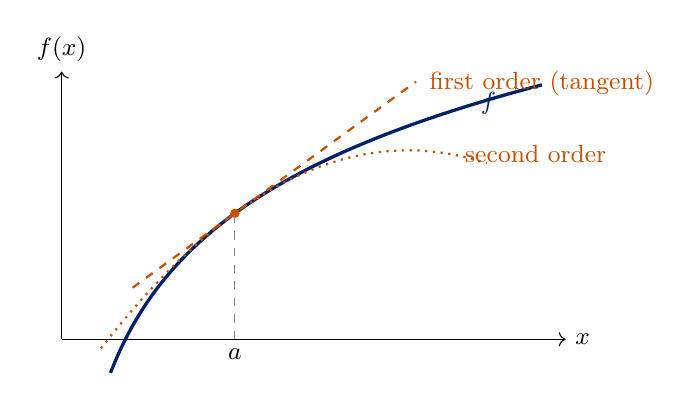
\begin{tikzpicture}[scale=1.0]
  \draw[->] (0,0) -- (6.4,0) node[right]{\small $x$};
  \draw[->] (0,0) -- (0,3.4) node[above]{\small $f(x)$};
  \draw[dukeblue,very thick,smooth,samples=100,domain=0.62:6.1,variable=\x]
    plot ({\x},{1.6+1.6*ln(\x/2.2)});
  \draw[accent,thick,dashed,domain=0.9:4.5,variable=\x]
    plot ({\x},{1.6+(1.6/2.2)*(\x-2.2)});
  \draw[accent,thick,dotted,thick,smooth,samples=100,domain=0.5:5.4,variable=\x]
    plot ({\x},{1.6+(1.6/2.2)*(\x-2.2)-(1.6/(2*2.2*2.2))*(\x-2.2)^2});
  \fill[accent] (2.2,1.6) circle (0.06);
  \draw[dashed,gray] (2.2,0) -- (2.2,1.6);
  \node[below] at (2.2,0) {\small $a$};
  \node[accent,anchor=west] at (4.55,3.25) {\small first order (tangent)};
  \node[accent,anchor=west] at (5.0,2.35) {\small second order};
  \node[dukeblue,anchor=west] at (5.2,3.0) {\small $f$};
\end{tikzpicture}
\end{center}

\begin{example}[Three expansions you can check on a calculator]
\begin{align*}
  e^{x} &\approx 1 + x + \tfrac12 x^2 && \text{around } a = 0;\ e^{0.1} = 1.1052,\ 1 + 0.1 + 0.005 = 1.105 \\
  \log(1+x) &\approx x - \tfrac12 x^2 && \text{around } a = 0;\ \log 1.1 = 0.0953,\ 0.1 - 0.005 = 0.095 \\
  \log x &\approx (x-1) - \tfrac12 (x-1)^2 && \text{around } a = 1 \text{ (the same fact, shifted)}
\end{align*}
For $e^x$ every derivative is $e^x$, which is $1$ at $0$. For $\log(1+x)$:
$f(0) = 0$, $f'(x) = 1/(1+x)$ so $f'(0) = 1$, $f''(x) = -1/(1+x)^2$ so
$f''(0) = -1$, hence the $-\tfrac12 x^2$.
\end{example}

The first-order version is used constantly under the name
\emph{linearization}: replace a curve by its tangent line and reason about
the line.

\begin{inthecourse}
\textbf{Percentage changes.} $\log(1+x) \approx x$ for small $x$ is why a
coefficient of $0.05$ on $\log$ earnings reads as ``about $5\%$.'' At
$0.5$ the approximation is poor: $e^{0.5} - 1 = 0.65$, not $0.50$.

\textbf{The delta method (Weeks 4 and 14).} If $\hat\theta$ has standard
error $\mathrm{se}$, then $g(\hat\theta) \approx g(\theta) +
g'(\theta)(\hat\theta - \theta)$, so $g(\hat\theta)$ has standard error
approximately $|g'(\theta)|\,\mathrm{se}$. Example: the standard error of
an odds ratio $e^{\hat\beta}$ is about $e^{\hat\beta}\,\mathrm{se}(\hat\beta)$,
because $\frac{\dd}{\dd\beta}e^{\beta} = e^{\beta}$. With several
parameters, $\Var(g(\hat{\bbeta})) \approx \nabla g'\,\Var(\hat{\bbeta})\,\nabla g$,
the rule of Section~\ref{sec:varlin} applied to the tangent plane.
\end{inthecourse}

\subsection{Taylor expansion at a maximum: why a parabola}
\label{sec:taylor-max}

Now expand the log-likelihood around its peak $\hat\theta$:
\begin{align*}
  \loglik(\theta) = \loglik(\hat\theta) + \loglik'(\hat\theta)\,(\theta-\hat\theta)
  + \frac{\loglik''(\hat\theta)}{2}\,(\theta-\hat\theta)^2
  + \frac{\loglik'''(\hat\theta)}{6}\,(\theta-\hat\theta)^3 + \cdots
\end{align*}
At the peak the slope is zero, $\loglik'(\hat\theta) = 0$, so the linear
term vanishes. The first term that carries any shape is the quadratic one.
Writing $\Info = -\loglik''(\hat\theta)$ for the observed information,
\begin{align*}
  \loglik(\theta) \approx \loglik(\hat\theta) - \frac{\Info}{2}\,(\theta-\hat\theta)^2 .
\end{align*}
This is the parabola that Week 3's testing section is built on. Two
consequences follow immediately.

\paragraph{The drop at $c$ standard errors is $c^2/2$.} Put
$\theta = \hat\theta + c\,\mathrm{se}$ with $\mathrm{se} = 1/\sqrt{\Info}$:
\begin{align*}
  \loglik(\hat\theta) - \loglik(\hat\theta + c\,\mathrm{se})
  \approx \frac{\Info}{2}\cdot\frac{c^2}{\Info} = \frac{c^2}{2}.
\end{align*}
So ``$1.96$ standard errors from the peak'' and ``$1.92 = 1.96^2/2$ below
the peak'' describe the same set of $\theta$ values, which is why the Wald
and likelihood-ratio tests agree whenever the parabola is accurate.

\paragraph{The error shrinks like $1/\sqrt n$.} The next term is
$\frac{1}{6}\loglik'''(\hat\theta)(c\,\mathrm{se})^3 =
\frac{c^3}{6}\,\loglik'''(\hat\theta)/\Info^{3/2}$. The log-likelihood is a
sum of $n$ terms, so $\loglik'''$ grows like $n$ while $\Info^{3/2}$ grows
like $n^{3/2}$; the ratio shrinks like $1/\sqrt n$. Within a few standard
errors of the peak, which is the only place a test looks, the curve becomes
a parabola as $n$ grows. That is the content of the ``Why Large $n$ Makes a
Parabola'' slide, and the reason $z$-tests work in large samples and fail in
small ones near a boundary.

\subsection{Newton's method: maximize the parabola instead}

If $\loglik$ has no closed-form maximum, use the parabola. Expand around
the current guess $\theta^{[t]}$ (not the peak, so the linear term stays):
\begin{align*}
  \loglik(\theta) \approx \loglik(\theta^{[t]}) + S(\theta^{[t]})(\theta - \theta^{[t]})
  + \frac{\loglik''(\theta^{[t]})}{2}(\theta - \theta^{[t]})^2 .
\end{align*}
The right-hand side is a parabola in $\theta$; maximize \emph{it} by
differentiating and setting to zero:
$S(\theta^{[t]}) + \loglik''(\theta^{[t]})(\theta - \theta^{[t]}) = 0$, so
\begin{align*}
  \theta^{[t+1]} = \theta^{[t]} - \frac{S(\theta^{[t]})}{\loglik''(\theta^{[t]})}
  = \theta^{[t]} + \frac{\text{slope}}{-\loglik''(\theta^{[t]})} .
\end{align*}
Step by slope over curvature, then repeat from the new point. Week 3's
``Poisson by Hand'' table is four rounds of this formula. With several
parameters the same derivation gives
$\bbeta^{[t+1]} = \bbeta^{[t]} - H^{-1}\nabla\loglik$, gradient and Hessian in
place of slope and curvature; that is what \texttt{glm()} and
\texttt{optim()} iterate.

\subsection{Several variables}

The second-order expansion around a point $\bm a$ uses the gradient and the
Hessian:
\begin{align*}
  f(\bbeta) \approx f(\bm a) + \nabla f(\bm a)'(\bbeta - \bm a)
  + \frac12(\bbeta - \bm a)'\,H(\bm a)\,(\bbeta - \bm a).
\end{align*}
The last term is a \emph{quadratic form}, defined in
Section~\ref{sec:quad}. Everything said above transfers: at a peak the
gradient is zero, the log-likelihood is locally a bowl-shaped-down
quadratic, and minus the Hessian is the information matrix whose inverse is
the variance matrix.

\begin{exercise}
Expand $f(\theta) = 5\log\theta - \theta$ to second order around $a = 5$
(its peak). Use it to estimate $f(4)$, and compare with the exact value.
\end{exercise}

\begin{takeaway}
Near a point, any smooth function is its tangent line, then its parabola.
At a peak the tangent is flat, so the parabola is the leading shape; its
curvature is the information, the drop at $c$ standard errors is $c^2/2$,
and the error shrinks like $1/\sqrt n$. Newton's method maximizes the
parabola repeatedly. The delta method is the tangent line applied to a
function of an estimate.
\end{takeaway}

%%%%%%%%%%%%%%%%%%%%%%%%%%%%%%%%%%%%%%%%%%%%%%%%%%%%%%%%%%%%%%%%%%%%%%%%%%%%%%%
\section{Linear algebra}
\label{sec:linalg}

\subsection{Vectors}

A vector is a list of numbers. In this course vectors are \textbf{columns}
unless stated otherwise, and a prime turns a column into a row (the
\textbf{transpose}):
\begin{align*}
  \bbeta = \begin{pmatrix}\beta_0\\ \beta_1\\ \beta_2\end{pmatrix},
  \qquad
  \bbeta' = \begin{pmatrix}\beta_0 & \beta_1 & \beta_2\end{pmatrix}.
\end{align*}
A vector with $k$ entries lives in $\R^k$. Vectors of the same length add
entry by entry, and a number times a vector scales every entry.

The \textbf{inner product} (dot product) of two vectors of the same length
multiplies matching entries and adds:
\begin{align*}
  \bm a'\bm b = \sum_{j=1}^{k} a_j b_j .
\end{align*}
It is a single number. This is the notation behind every regression line in
the course. If $X_i = (1, x_{i1}, x_{i2})'$ holds person $i$'s covariates
(a leading $1$ for the intercept), then
\begin{align*}
  X_i'\bbeta = \beta_0 + \beta_1 x_{i1} + \beta_2 x_{i2}
\end{align*}
is the linear predictor for that person. Reading $X_i'\bbeta$ as
``the weighted sum of $i$'s covariates'' should become automatic.

The \textbf{length} (norm) of a vector is $\|\bm a\| = \sqrt{\bm a'\bm a} =
\sqrt{\sum_j a_j^2}$. Two vectors are \textbf{orthogonal} when their inner
product is zero. The OLS normal equations say that the residual vector is
orthogonal to every column of $X$.

\subsection{Matrices}

A matrix is a rectangular array with $r$ rows and $c$ columns, written
$A$ is $r \times c$. Entry $(i,j)$ sits in row $i$, column $j$. The
transpose $A'$ flips rows and columns, so it is $c \times r$, and
$(A')' = A$.

\paragraph{Multiplication.} $AB$ is defined only when the number of
columns of $A$ equals the number of rows of $B$. If $A$ is $r \times m$
and $B$ is $m \times c$, then $AB$ is $r \times c$, and entry $(i,j)$ of
$AB$ is the inner product of row $i$ of $A$ with column $j$ of $B$:
\begin{align*}
  (AB)_{ij} = \sum_{l=1}^{m} A_{il}B_{lj} .
\end{align*}

\begin{example}
\begin{align*}
  \begin{pmatrix} 1 & 2 \\ 3 & 4 \end{pmatrix}
  \begin{pmatrix} 5 & 0 \\ 1 & 2 \end{pmatrix}
  =
  \begin{pmatrix} 1\cdot5 + 2\cdot1 & 1\cdot0 + 2\cdot2 \\ 3\cdot5 + 4\cdot1 & 3\cdot0 + 4\cdot2 \end{pmatrix}
  =
  \begin{pmatrix} 7 & 4 \\ 19 & 8 \end{pmatrix}.
\end{align*}
Reverse the order and you get a different answer:
$\begin{pmatrix} 5 & 0 \\ 1 & 2 \end{pmatrix}\begin{pmatrix} 1 & 2 \\ 3 & 4 \end{pmatrix}
= \begin{pmatrix} 5 & 10 \\ 7 & 10 \end{pmatrix}$. Matrix multiplication is
\textbf{not commutative}: $AB \ne BA$ in general. It is associative,
$(AB)C = A(BC)$, and distributes over addition.
\end{example}

\begin{rulebox}[transpose of a product]
$(AB)' = B'A'$: transpose each factor and reverse the order.
\end{rulebox}

The \textbf{identity matrix} $I$ has ones on the diagonal and zeros
elsewhere; $AI = IA = A$. A matrix is \textbf{symmetric} when $A' = A$;
$X'X$ is always symmetric, since $(X'X)' = X'(X')' = X'X$. A
\textbf{diagonal} matrix has zeros off the diagonal; $\lambda I$ is the
diagonal matrix with $\lambda$ everywhere on the diagonal (Week 12's ridge
penalty).

\subsection{The data as a matrix}

Stack the $n$ covariate vectors as rows and the $n$ outcomes as a column:
\begin{align*}
  \X = \begin{pmatrix} X_1' \\ X_2' \\ \vdots \\ X_n' \end{pmatrix}
  = \begin{pmatrix}
      1 & x_{11} & x_{12} \\
      1 & x_{21} & x_{22} \\
      \vdots & \vdots & \vdots \\
      1 & x_{n1} & x_{n2}
    \end{pmatrix}
  \ (n \times k),
  \qquad
  \Y = \begin{pmatrix} y_1 \\ y_2 \\ \vdots \\ y_n \end{pmatrix}
  \ (n \times 1).
\end{align*}
Then three products do all the work in the course:
\begin{itemize}
  \item $\X\bbeta$ is $n \times 1$: row $i$ is $X_i'\bbeta$, so $\X\bbeta$
        is the vector of all $n$ linear predictors at once, and
        $\Y - \X\bbeta$ is the vector of residuals.
  \item $\X'\X$ is $k \times k$: entry $(j,l)$ is $\sum_i x_{ij}x_{il}$, a
        sum of cross-products over people. Equivalently $\X'\X = \sum_i
        X_iX_i'$, a sum of $n$ little $k \times k$ matrices, one per
        person. This is why information ``adds up'' across observations.
  \item $\X'\Y$ is $k \times 1$: entry $j$ is $\sum_i x_{ij}y_i$.
\end{itemize}

\begin{example}[Check the dimensions before anything else]
$\X'$ is $k \times n$, $\X$ is $n \times k$, so $\X'\X$ is $k \times k$.
$\X'\Y$ is $(k \times n)(n \times 1) = k \times 1$. And $(\X'\X)^{-1}\X'\Y$
is $(k\times k)(k \times 1) = k \times 1$: one number per coefficient, as it
must be. If the dimensions do not line up, the expression is wrong.
\end{example}

\subsection{The inverse}

The inverse of a square matrix $A$, written $A^{-1}$, is the matrix with
$A^{-1}A = AA^{-1} = I$. It plays the role of division: the solution of
$A\bbeta = \bm c$ is $\bbeta = A^{-1}\bm c$, just as the solution of
$5\beta = 10$ is $\beta = 5^{-1}\cdot 10$.

For a $2 \times 2$ matrix,
\begin{align*}
  \begin{pmatrix} a & b \\ c & d \end{pmatrix}^{-1}
  = \frac{1}{ad - bc}\begin{pmatrix} d & -b \\ -c & a \end{pmatrix},
\end{align*}
which exists only when $ad - bc \ne 0$. Larger inverses are left to the
computer (\texttt{solve()} in R).

\paragraph{When the inverse does not exist.} A matrix is
\textbf{singular} (no inverse) when one of its columns is a linear
combination of the others, so that the columns carry redundant information.
For $\X'\X$ this happens exactly when the columns of $\X$ are linearly
dependent: a dummy for female plus a dummy for male, both with an intercept;
or a variable in both dollars and thousands of dollars. That is
\textbf{perfect collinearity}, and the regression has no unique solution.
The \textbf{rank} of a matrix is the number of linearly independent
columns; $\X'\X$ is invertible if and only if $\X$ has full column rank
$k$. R drops a column and reports \texttt{NA} when it is not; Lab 3's
non-identification example is the same phenomenon in a likelihood.

\begin{rulebox}[inverse of a product]
$(AB)^{-1} = B^{-1}A^{-1}$, reversed order, when both inverses exist. Also
$(A')^{-1} = (A^{-1})'$, and the inverse of a symmetric matrix is
symmetric.
\end{rulebox}

\subsection{Projection, and the Frisch--Waugh--Lovell idea}
\label{sec:projection}

Multiplying $\Y$ by $P = \X(\X'\X)^{-1}\X'$ gives the fitted values
$\hat{\Y} = \X\bhat$; multiplying by $M = I - P$ gives the residuals
$\Y - \hat{\Y}$. $P$ is called a \textbf{projection matrix}: it drops $\Y$
onto the space spanned by the columns of $\X$, and applying it twice
changes nothing ($PP = P$). Two facts are used repeatedly in Weeks 10 and
13:
\begin{itemize}
  \item $M\X = \bm 0$: residualizing a variable on $\X$ removes everything
        in $\X$ from it.
  \item \textbf{Frisch--Waugh--Lovell.} In a regression of $\Y$ on
        $\X_1$ and $\X_2$, the coefficient on $\X_2$ equals the coefficient
        from regressing the residual of $\Y$ on $\X_1$ against the residual
        of $\X_2$ on $\X_1$. ``Holding $\X_1$ constant'' means ``after
        removing $\X_1$ from both.'' Fixed effects (Week 10) are FWL with
        group dummies as $\X_1$; double machine learning (Week 13) is FWL
        with the two residualizations done by a flexible learner.
\end{itemize}

\subsection{Quadratic forms, positive definiteness}
\label{sec:quad}

For a symmetric $k \times k$ matrix $A$ and a vector $\bbeta$, the
\textbf{quadratic form} $\bbeta'A\bbeta$ is a single number,
\begin{align*}
  \bbeta'A\bbeta = \sum_{j=1}^{k}\sum_{l=1}^{k} A_{jl}\,\beta_j\beta_l ,
\end{align*}
the matrix version of $a\beta^2$. In two dimensions,
$\bbeta'A\bbeta = A_{11}\beta_1^2 + 2A_{12}\beta_1\beta_2 + A_{22}\beta_2^2$.

$A$ is \textbf{positive definite} when $\bbeta'A\bbeta > 0$ for every
$\bbeta \ne \bm 0$, and \textbf{negative definite} when the inequality is
reversed. These are the matrix versions of a positive and a negative number.
Three places you meet them:
\begin{itemize}
  \item A variance matrix is positive definite (a variance of a nonzero
        combination of estimates is positive).
  \item $\X'\X$ is positive definite when $\X$ has full column rank,
        because $\bbeta'\X'\X\bbeta = (\X\bbeta)'(\X\bbeta) = \|\X\bbeta\|^2
        > 0$.
  \item The Hessian at a maximum is negative definite: the log-likelihood
        bends down in every direction. Minus the Hessian, the information
        matrix, is positive definite, and its inverse, the variance matrix,
        is too.
\end{itemize}
The sum of squared residuals is a quadratic form:
$\sum_i (y_i - X_i'\bbeta)^2 = (\Y - \X\bbeta)'(\Y - \X\bbeta)$.

\subsection{Derivatives with respect to a vector}
\label{sec:matcalc}

Differentiating with respect to a vector means collecting the partial
derivatives with respect to each entry into a column, which is the gradient
of Section~\ref{sec:partial}. Two rules cover OLS and ridge.

\begin{rulebox}[vector derivatives]
For a constant vector $\bm a$ and a constant symmetric matrix $A$,
\begin{align*}
  \frac{\partial}{\partial\bbeta}\,(\bm a'\bbeta) = \bm a,
  \qquad\qquad
  \frac{\partial}{\partial\bbeta}\,(\bbeta'A\bbeta) = 2A\bbeta .
\end{align*}
\end{rulebox}
The first is the vector version of $\frac{\dd}{\dd\beta}(a\beta) = a$; the
second of $\frac{\dd}{\dd\beta}(a\beta^2) = 2a\beta$. To see the first,
$\bm a'\bbeta = \sum_j a_j\beta_j$, and its partial with respect to
$\beta_j$ is $a_j$; stack them and you have $\bm a$.

\begin{example}[OLS in matrix form, derived]
Minimize the sum of squared residuals $Q(\bbeta) = (\Y - \X\bbeta)'(\Y -
\X\bbeta)$. First multiply it out, using $(AB)' = B'A'$ and the fact that
$\Y'\X\bbeta$ is a $1 \times 1$ matrix, hence equal to its own transpose
$\bbeta'\X'\Y$:
\begin{align*}
  Q(\bbeta) = \Y'\Y - 2\,\bbeta'\X'\Y + \bbeta'\X'\X\bbeta .
\end{align*}
Now differentiate with the two rules (constant vector $\bm a = \X'\Y$,
constant symmetric matrix $A = \X'\X$):
\begin{align*}
  \frac{\partial Q}{\partial\bbeta} = -2\,\X'\Y + 2\,\X'\X\bbeta .
\end{align*}
Set it to zero (the first-order condition) and solve, which needs the
inverse to exist:
\begin{align*}
  \X'\X\bbeta = \X'\Y \qquad\Longrightarrow\qquad \bhat = (\X'\X)^{-1}\X'\Y .
\end{align*}
These are the \textbf{normal equations}. Rewriting the first form as
$\X'(\Y - \X\bhat) = \bm 0$ says the residual vector is orthogonal to every
column of $\X$, the several-variable version of the one-parameter example
in Section~\ref{sec:max}. The Hessian is $\partial^2 Q/\partial\bbeta\,\partial\bbeta'
= 2\X'\X$, positive definite when $\X$ has full column rank, so this is a
minimum. This is Week 1's derivation.
\end{example}

\subsection{Variances of linear combinations}
\label{sec:varlin}

The last rule turns a variance matrix of one vector into the variance matrix
of a linear transformation of it.

\begin{rulebox}[variance of $A\bm u$]
If $\bm u$ is a random vector with variance matrix $\Var(\bm u)$ and $A$
is a constant matrix, then $\Var(A\bm u) = A\,\Var(\bm u)\,A'$.
\end{rulebox}
The scalar version is $\Var(au) = a^2\Var(u)$; the matrix version keeps
one $A$ on each side because the result must be symmetric.

\begin{example}[The OLS variance matrix]
Write $\Y = \X\bbeta + \bm\epsilon$ with $\Var(\bm\epsilon) = \sigma^2 I$
(constant variance, no correlation). Then
$\bhat = (\X'\X)^{-1}\X'\Y = \bbeta + (\X'\X)^{-1}\X'\bm\epsilon$, so with
$A = (\X'\X)^{-1}\X'$,
\begin{align*}
  \Var(\bhat) = A\,(\sigma^2 I)\,A'
  = \sigma^2 (\X'\X)^{-1}\X'\X(\X'\X)^{-1}
  = \sigma^2(\X'\X)^{-1},
\end{align*}
using $A' = \X(\X'\X)^{-1}$ (transpose reverses order; the inverse of a
symmetric matrix is symmetric) and then cancelling $\X'\X$ against one
inverse. The standard errors in every regression table are the square roots
of the diagonal of this matrix with $s^2$ in place of $\sigma^2$. If
$\Var(\bm\epsilon)$ is not $\sigma^2 I$, the middle no longer cancels and
you are left with $(\X'\X)^{-1}\X'\,\Var(\bm\epsilon)\,\X(\X'\X)^{-1}$: the
sandwich of Week 2, with the robust estimator filling in the middle.
\end{example}

\begin{exercise}
Let $\X = \begin{pmatrix} 1 & 0 \\ 1 & 1 \\ 1 & 2 \end{pmatrix}$ and
$\Y = (1, 2, 4)'$. Compute $\X'\X$, $\X'\Y$, $(\X'\X)^{-1}$ with the
$2\times2$ formula, and $\bhat$. Check that the residuals sum to zero.
\end{exercise}

\begin{takeaway}
$X_i'\bbeta$ is a weighted sum; $\X\bbeta$ is all of them at once;
$\X'\X$ adds up cross-products over people; the inverse undoes a matrix
when the columns are not redundant; $P$ projects and $M$ residualizes; two
vector-derivative rules give the normal equations; $\Var(A\bm u) =
A\Var(\bm u)A'$ gives every standard error and the sandwich.
\end{takeaway}

%%%%%%%%%%%%%%%%%%%%%%%%%%%%%%%%%%%%%%%%%%%%%%%%%%%%%%%%%%%%%%%%%%%%%%%%%%%%%%%
\section{Probability: expectation, variance, covariance}
\label{sec:prob}

From Week 5 the objects of interest are population quantities such as
$\E[Y(1)] - \E[Y(0)]$ and the proofs are a few lines of expectation
algebra. This section is that algebra.

\subsection{Expectation}

A random variable $Y$ takes values with probabilities. Its
\textbf{expectation} $\E[Y]$ is the probability-weighted average of the
values: for a discrete $Y$, $\E[Y] = \sum_y y\,\Pr(Y = y)$; for a
continuous one, an integral (Section~\ref{sec:integrals}). The sample mean
$\bar y$ is the data version, with each observed value weighted $1/n$.

\begin{rulebox}[linearity of expectation]
For constants $a, b$ and any random variables $X, Y$, related or not,
\begin{align*}
  \E[a + bY] = a + b\,\E[Y], \qquad\qquad \E[X + Y] = \E[X] + \E[Y].
\end{align*}
\end{rulebox}
This is the single most used fact in the course: an expectation goes
through sums and constants. It does \emph{not} go through products or
nonlinear functions: $\E[XY] \ne \E[X]\E[Y]$ in general, and $\E[\log Y]
\ne \log\E[Y]$ (Jensen's inequality says $\E[\log Y] < \log\E[Y]$, which is
why a regression of $\log$ earnings does not model mean earnings).

\paragraph{Indicators.} For an event $A$, the indicator $\ind\{A\}$ is $1$
when $A$ happens and $0$ otherwise. Its expectation is the probability:
$\E[\ind\{A\}] = 1\cdot\Pr(A) + 0\cdot\Pr(\text{not }A) = \Pr(A)$. A
treatment dummy $D$ is an indicator, so $\E[D] = \Pr(D = 1)$ is the share
treated; a binary outcome $Y$ has $\E[Y] = \Pr(Y = 1)$, which is why a
logit models a probability by modelling a mean.

\subsection{Variance and covariance}

\begin{align*}
  \Var(Y) &= \E\big[(Y - \E[Y])^2\big] = \E[Y^2] - (\E[Y])^2, \\
  \Cov(X, Y) &= \E\big[(X - \E[X])(Y - \E[Y])\big] = \E[XY] - \E[X]\E[Y].
\end{align*}
Variance is the average squared distance from the mean; covariance is the
average product of the two deviations, positive when $X$ and $Y$ tend to be
above or below their means together. $\Cov(Y, Y) = \Var(Y)$, and the
correlation is $\Cov(X,Y)/\sqrt{\Var(X)\Var(Y)}$.

\begin{rulebox}[variance and covariance algebra]
For constants $a, b, c$,
\begin{align*}
  \Var(a + bY) &= b^2\Var(Y), \\
  \Cov(a + bX,\ c + dY) &= bd\,\Cov(X, Y), \\
  \Cov(X + Z,\ Y) &= \Cov(X, Y) + \Cov(Z, Y), \\
  \Var(X + Y) &= \Var(X) + \Var(Y) + 2\Cov(X, Y), \\
  \Var(X + Y) &= \Var(X) + \Var(Y) \quad\text{if } \Cov(X, Y) = 0 .
\end{align*}
\end{rulebox}
In words: shifting does nothing to a variance and scaling squares;
covariance is bilinear and goes through sums; the variance of a sum picks
up a cross term that vanishes when the two are uncorrelated.
The last line, applied to $n$ independent draws each with variance
$\sigma^2$, gives $\Var(\sum_i y_i) = n\sigma^2$, hence
$\Var(\bar y) = \Var(\frac1n\sum_i y_i) = \frac{1}{n^2}\cdot n\sigma^2 =
\sigma^2/n$: the standard error of a mean shrinks like $1/\sqrt n$. Every
standard error in the course descends from this line.

\begin{example}[Regression slopes are covariance ratios, Week 1]
With one regressor, $\hat\beta_1 = \widehat\Cov(X, Y)/\widehat\Var(X)$.
If $Y = \beta_0 + \beta_1 X + \epsilon$ with $\Cov(X, \epsilon) = 0$, then
$\Cov(X, Y) = \Cov(X, \beta_0 + \beta_1 X + \epsilon) = \beta_1\Var(X) +
\Cov(X, \epsilon) = \beta_1\Var(X)$, using bilinearity and that a constant
has zero covariance with anything. So $\Cov(X,Y)/\Var(X) = \beta_1$. If
$\Cov(X, \epsilon) \ne 0$ (an omitted variable), the ratio is
$\beta_1 + \Cov(X,\epsilon)/\Var(X)$: the omitted-variable bias formula.
\end{example}

\begin{example}[The instrumental-variables estimand, Week 7]
Take $\Cov$ with an instrument $Z$ instead of with $X$ itself. From
$Y = \beta_0 + \beta_1 D + \epsilon$,
\begin{align*}
  \Cov(Z, Y) = \beta_1\Cov(Z, D) + \Cov(Z, \epsilon) = \beta_1\Cov(Z, D)
  \qquad\Longrightarrow\qquad
  \beta_1 = \frac{\Cov(Z, Y)}{\Cov(Z, D)},
\end{align*}
provided the instrument is uncorrelated with the error (exclusion,
$\Cov(Z,\epsilon) = 0$) and moves the treatment (relevance,
$\Cov(Z, D) \ne 0$). Two lines of covariance algebra are the whole IV
identification argument.
\end{example}

\subsection{Independence and mean independence}

$X$ and $Y$ are \textbf{independent} when knowing one tells you nothing
about the distribution of the other: $\Pr(Y \le y \mid X = x)$ does not
depend on $x$. Independence implies $\Cov(X, Y) = 0$, but zero covariance
does not imply independence (covariance sees only linear association). A
weaker and often sufficient condition is \textbf{mean independence},
$\E[Y \mid X] = \E[Y]$: the mean of $Y$ does not move with $X$, whatever
the rest of its distribution does. Week 5's ``ignorability,''
$Y(0), Y(1) \perp\!\!\!\perp D \mid X$, is a conditional independence; what
the estimators actually use is the mean version,
$\E[Y(d) \mid D, X] = \E[Y(d) \mid X]$.

\begin{takeaway}
Expectations go through sums and constants, never through products or
nonlinear functions. Variance squares a scale factor; covariance is
bilinear; the variance of a sum picks up a cross term that vanishes under
independence, which is where $\sigma^2/n$ and every standard error come
from. A regression slope is a covariance ratio; so is the IV estimand.
\end{takeaway}

%%%%%%%%%%%%%%%%%%%%%%%%%%%%%%%%%%%%%%%%%%%%%%%%%%%%%%%%%%%%%%%%%%%%%%%%%%%%%%%
\section{Conditional expectation and iterated expectations}
\label{sec:condexp}

\subsection{The conditional expectation function}

$\E[Y \mid X = x]$ is the mean of $Y$ among units with $X = x$. As $x$
varies it traces a function of $x$, the \textbf{conditional expectation
function} (CEF), written $\E[Y \mid X]$. It is the object regression
approximates: Week 1's line is the best linear approximation to the CEF, a
logit is a CEF for a binary $Y$, and Week 5's treatment effect is a
difference of two CEFs, $\E[Y \mid D = 1, X] - \E[Y \mid D = 0, X]$.

Two properties:
\begin{itemize}
  \item Inside a conditional expectation, anything that is a function of
        the conditioning variable acts like a constant: $\E[g(X)\,Y \mid X]
        = g(X)\,\E[Y \mid X]$. Given $X$, $g(X)$ is known.
  \item The conditional expectation is itself a random variable (it
        depends on $X$), so it has an expectation of its own. That is the
        next rule.
\end{itemize}

\subsection{The law of iterated expectations}

\begin{rulebox}[iterated expectations]
\begin{align*}
  \E\big[\E[Y \mid X]\big] = \E[Y].
\end{align*}
Average $Y$ within each value of $X$, then average those averages over the
distribution of $X$: you get the overall average. More generally
$\E[\E[Y \mid X, Z] \mid X] = \E[Y \mid X]$: conditioning on more and then
averaging it back out returns the coarser conditioning.
\end{rulebox}

This rule is the engine of every identification proof from Week 5 on.
The pattern is always the same: write the quantity you want as an
expectation, condition on something that makes it computable, then average
back out.

\begin{example}[The average treatment effect under ignorability, Week 5]
Suppose $\E[Y(1) \mid D, X] = \E[Y(1) \mid X]$ (within strata of $X$,
treatment is as good as random). Then the mean potential outcome under
treatment is
\begin{align*}
  \E[Y(1)] = \E\big[\E[Y(1) \mid X]\big] = \E\big[\E[Y(1) \mid D = 1, X]\big]
  = \E\big[\E[Y \mid D = 1, X]\big].
\end{align*}
First equality: iterated expectations. Second: the assumption. Third: among
the treated, $Y(1)$ is the observed $Y$. The right-hand side involves only
observable quantities: the mean outcome of the treated in each stratum,
averaged over the whole population's $X$ distribution. That is what
regression adjustment, matching, and Week 4's observed-value predictions
compute.
\end{example}

\begin{example}[Inverse probability weighting, Week 6]
Let $e(X) = \Pr(D = 1 \mid X) = \E[D \mid X]$ be the propensity score.
Then
\begin{align*}
  \E\!\left[\frac{D\,Y}{e(X)}\right]
  &= \E\!\left[\E\!\left[\frac{D\,Y(1)}{e(X)} \,\Big|\, X\right]\right]
  = \E\!\left[\frac{\E[D\,Y(1) \mid X]}{e(X)}\right] \\
  &= \E\!\left[\frac{\E[D \mid X]\,\E[Y(1) \mid X]}{e(X)}\right]
  = \E\big[\E[Y(1) \mid X]\big] = \E[Y(1)].
\end{align*}
Step 1: iterated expectations, and $DY = DY(1)$ because $D = 1$ whenever
the product is nonzero. Step 2: $e(X)$ is a function of $X$, so it comes
out of the inner expectation. Step 3: ignorability makes $D$ and $Y(1)$
mean-independent given $X$, so the expectation of the product is the
product of expectations. Step 4: $\E[D \mid X] = e(X)$ cancels. Step 5:
iterated expectations again. Weighting each treated unit by $1/e(X)$
recovers the mean of $Y(1)$ for everyone.
\end{example}

\subsection{Bayes' rule and the propensity score}

\begin{rulebox}[Bayes]
$\Pr(A \mid B) = \dfrac{\Pr(B \mid A)\,\Pr(A)}{\Pr(B)}$.
\end{rulebox}
The propensity score $e(X) = \Pr(D = 1 \mid X)$ is a conditional
probability of this kind, estimated in practice by a logit of $D$ on $X$.
Bayes' rule is also why the score works as a summary of $X$: conditional on
$e(X)$, the distribution of $X$ is the same in the treated and control
groups (Rosenbaum and Rubin's balancing property, Week 6), because
$\Pr(D = 1 \mid X, e(X)) = e(X)$ does not depend on $X$ beyond $e(X)$.

\subsection{Conditional variance, and the bias--variance decomposition}

$\Var(Y \mid X)$ is the variance within a value of $X$. The law of total
variance, $\Var(Y) = \E[\Var(Y \mid X)] + \Var(\E[Y \mid X])$, splits the
overall variance into a within part and a between part; $R^2$ is the second
term's share.

The same decomposition applied to an estimator gives the formula Week 12
lives on. For an estimator $\hat\theta$ of a target $\theta$,
\begin{align*}
  \E\big[(\hat\theta - \theta)^2\big]
  = \big(\E[\hat\theta] - \theta\big)^2 + \Var(\hat\theta)
  = \text{bias}^2 + \text{variance}.
\end{align*}
To see it, add and subtract $\E[\hat\theta]$ inside the square, expand, and
note that the cross term $2(\E[\hat\theta] - \theta)\,\E[\hat\theta -
\E[\hat\theta]]$ is zero because $\E[\hat\theta - \E[\hat\theta]] = 0$.
Ridge and lasso accept a little bias to buy a large drop in variance.

\begin{exercise}
Let $D$ be a treatment dummy with $\Pr(D = 1) = p$, and suppose
$\E[Y \mid D = 1] = 5$ and $\E[Y \mid D = 0] = 3$. Use iterated
expectations to write $\E[Y]$ in terms of $p$, and evaluate it at
$p = 0.25$.
\end{exercise}

\begin{takeaway}
The CEF is what regression estimates; inside $\E[\cdot \mid X]$, functions
of $X$ are constants; iterated expectations lets you condition on what
makes a quantity computable and average back out, which is the shape of
every identification proof; Bayes' rule is the propensity score; mean
squared error is bias squared plus variance.
\end{takeaway}

%%%%%%%%%%%%%%%%%%%%%%%%%%%%%%%%%%%%%%%%%%%%%%%%%%%%%%%%%%%%%%%%%%%%%%%%%%%%%%%
\section{Limits and asymptotics}
\label{sec:asymp}

\subsection{What ``as $n \to \infty$'' means}

Almost every guarantee in the course is a statement about what an
estimator does as the sample grows. Three results carry all of them.

\begin{rulebox}[law of large numbers]
If $y_1, \dots, y_n$ are independent draws with mean $\mu$, then
$\bar y \pto \mu$: the sample mean converges in probability to the
population mean. Written $\plim \bar y = \mu$.
\end{rulebox}
``Converges in probability'' means: for any tolerance you name, the chance
that $\bar y$ misses $\mu$ by more than that tolerance goes to zero as $n$
grows. Since $\Var(\bar y) = \sigma^2/n \to 0$, the sample mean is pinned
ever more tightly to $\mu$. The same holds for any sample average, of
$y_i^2$, of $x_iy_i$, of $\log f(y_i \mid \theta)$: averages settle down.

\begin{rulebox}[central limit theorem]
Under the same conditions,
\begin{align*}
  \sqrt n\,(\bar y - \mu) \dto \mathcal N(0, \sigma^2),
  \qquad\text{equivalently}\qquad
  \bar y \overset{a}{\sim} \mathcal N\!\Big(\mu, \frac{\sigma^2}{n}\Big).
\end{align*}
\end{rulebox}
Whatever the shape of the $y_i$, the sampling distribution of the mean is
approximately normal once $n$ is large. The $\sqrt n$ is the rate: the
error $\bar y - \mu$ shrinks like $1/\sqrt n$, so multiplying by $\sqrt n$
holds it at a stable size, which is what lets a limit exist.

\begin{rulebox}[plug-in: continuous mapping and Slutsky]
If $\hat a \pto a$ and $\hat b \pto b$, then $g(\hat a, \hat b) \pto g(a,
b)$ for any continuous $g$ (ratios, products, logs, inverses). And if
$\sqrt n(\hat a - a) \dto \mathcal N(0, v)$ while $\hat b \pto b$, then
$\hat b\,\sqrt n(\hat a - a) \dto \mathcal N(0, b^2 v)$: a consistently
estimated constant can be plugged in without changing the limit.
\end{rulebox}

\begin{example}[Why OLS is consistent, Week 2]
$\hat\beta_1 = \widehat\Cov(X,Y)/\widehat\Var(X)$ is a ratio of two sample
averages. By the law of large numbers the numerator $\pto \Cov(X,Y)$ and
the denominator $\pto \Var(X)$; by continuous mapping the ratio
$\pto \Cov(X,Y)/\Var(X) = \beta_1$ when $\Cov(X, \epsilon) = 0$. The same
argument with $Z$ in place of $X$ gives consistency of the IV estimator in
Week 7.
\end{example}

\begin{example}[Why the MLE is asymptotically normal, Week 3]
Week 3's Newton step from the truth,
$\hat\theta - \theta_0 \approx S(\theta_0)/(-\loglik''(\theta_0))$, has a
sum of $n$ independent terms in the numerator (the score) and a sum in the
denominator (the curvature). Divide both by $n$: the numerator is an
average with mean zero, so by the CLT $\sqrt n$ times it is normal; the
denominator is an average that converges to the information per
observation by the LLN. Slutsky combines them:
$\sqrt n(\hat\theta - \theta_0) \dto \mathcal N(0, 1/\Info_1)$. Every
``the MLE is approximately normal with variance one over the information''
is this argument.
\end{example}

\subsection{What the limits do not say}

A limit theorem says nothing about any particular $n$. Week 3's
simulations show the normal approximation excellent at $n = 200$ for a
Poisson mean and useless at $n = 20$ for a rare Bernoulli; ``large enough''
depends on how far the finite-sample distribution is from its limit, which
is a question for simulation, not for the theorem. Two habits follow:
treat asymptotic standard errors as approximations, and when the sample or
the number of events is small, check by simulation or use an exact method.

\begin{takeaway}
Averages settle down (LLN) and their errors are normal at rate $1/\sqrt n$
(CLT); anything continuous in consistent pieces is consistent, and
consistent constants can be plugged in (Slutsky). OLS, IV, and the MLE are
all ``a ratio of averages,'' which is why the same three results cover all
of them.
\end{takeaway}

%%%%%%%%%%%%%%%%%%%%%%%%%%%%%%%%%%%%%%%%%%%%%%%%%%%%%%%%%%%%%%%%%%%%%%%%%%%%%%%
\section{Integrals, densities, and kernels}
\label{sec:integrals}

\subsection{The integral as an area and as a sum}

$\int_a^b f(x)\,\dd x$ is the area under $f$ between $a$ and $b$, or
equivalently the limit of a sum of thin rectangles of height $f(x)$ and
width $\dd x$. The integral is the reverse of the derivative (the
fundamental theorem of calculus): if $F'(x) = f(x)$ then $\int_a^b f(x)\,\dd
x = F(b) - F(a)$. So $\int_a^b e^{x}\,\dd x = e^{b} - e^{a}$ and $\int_a^b
\frac1x\,\dd x = \log b - \log a$.

For a continuous random variable, a \textbf{density} $f(y)$ is a curve
whose area over an interval is the probability of landing there,
$\Pr(a \le Y \le b) = \int_a^b f(y)\,\dd y$, with total area one. The
expectation is the density-weighted average $\E[Y] = \int y\,f(y)\,\dd y$,
the continuous version of $\sum_y y\Pr(Y = y)$; every rule of
Section~\ref{sec:prob} holds with integrals in place of sums. The
\textbf{cumulative distribution function} $F(y) = \Pr(Y \le y) =
\int_{-\infty}^{y} f(u)\,\dd u$ has derivative $F'(y) = f(y)$. The normal
CDF $\Phi$ and the logistic CDF $\Lambda$ of Week 4 are of this kind;
Example~\ref{ex:logistic-deriv} computed the logistic density.

\subsection{Survival and hazard, Week 4}

For a duration $T$ with density $f(t)$ and CDF $F(t)$, the
\textbf{survival function} is $S(t) = \Pr(T > t) = 1 - F(t)$, so
$S'(t) = -f(t)$. The \textbf{hazard} is the event rate among those still
at risk, $h(t) = f(t)/S(t)$. Since $f = -S'$,
\begin{align*}
  h(t) = -\frac{S'(t)}{S(t)} = -\frac{\dd}{\dd t}\log S(t)
  \qquad\Longrightarrow\qquad
  S(t) = \exp\!\Big(-\int_0^{t} h(u)\,\dd u\Big),
\end{align*}
using the chain rule for $\log S$ in the first step and the fundamental
theorem (with $S(0) = 1$, so $\log S(0) = 0$) in the second. Survival is the
exponential of minus the accumulated hazard; either function determines the
other, which is why models are written on the hazard scale and plotted on
the survival scale. The censored-data likelihood of Week 4 then uses $f(t)
= h(t)S(t)$ for observed events and $S(t)$ for censored ones.

\subsection{Kernels and local averaging, Week 9}

A \textbf{kernel} $K(u)$ is a symmetric bump that integrates to one,
$\int K(u)\,\dd u = 1$, such as the triangular kernel $K(u) = (1 -
|u|)\ind\{|u| \le 1\}$. A kernel-weighted average around a point $c$ with
bandwidth $h$ gives weight $K\big((x_i - c)/h\big)$ to observation $i$:
full weight at $c$, zero beyond $c \pm h$. Regression discontinuity
estimates the CEF just to the left and just to the right of a cutoff by
running weighted least squares with these weights (local linear
regression); the bandwidth $h$ trades bias (large $h$ averages in
far-away, different units) against variance (small $h$ uses few units),
the decomposition of Section~\ref{sec:condexp}. The kernel is just a
weighting rule; no new calculus is involved.

\begin{takeaway}
An integral is an area and a limit of sums; densities integrate to one and
expectations integrate against them; $S = \exp(-\int h)$ links survival to
hazard through the chain rule; a kernel is a weight that adds to one.
\end{takeaway}

%%%%%%%%%%%%%%%%%%%%%%%%%%%%%%%%%%%%%%%%%%%%%%%%%%%%%%%%%%%%%%%%%%%%%%%%%%%%%%%
\section{Constrained and penalized optimization}
\label{sec:constrained}

\subsection{Penalties: ridge and lasso, Week 12}

Least squares can be pushed toward smaller coefficients by adding a
\textbf{penalty} to the objective:
\begin{align*}
  \text{ridge:}&\quad \min_{\bbeta}\ (\Y - \X\bbeta)'(\Y - \X\bbeta) + \lambda\,\bbeta'\bbeta, \\
  \text{lasso:}&\quad \min_{\bbeta}\ (\Y - \X\bbeta)'(\Y - \X\bbeta) + \lambda\sum_j|\beta_j| .
\end{align*}
The tuning parameter $\lambda \ge 0$ is the price per unit of coefficient
size; $\lambda = 0$ is OLS, and larger $\lambda$ shrinks harder.

\begin{example}[Ridge in closed form]
The penalty $\lambda\bbeta'\bbeta = \bbeta'(\lambda I)\bbeta$ is a
quadratic form with the symmetric matrix $\lambda I$, so the vector
derivative rule gives $\partial(\lambda\bbeta'\bbeta)/\partial\bbeta =
2\lambda\bbeta$. Adding it to the OLS gradient of
Section~\ref{sec:matcalc}:
\begin{align*}
  -2\X'\Y + 2\X'\X\bbeta + 2\lambda\bbeta = \bm 0
  \qquad\Longrightarrow\qquad
  \bhat_{\text{ridge}} = (\X'\X + \lambda I)^{-1}\X'\Y .
\end{align*}
Two things to notice. The matrix $\X'\X + \lambda I$ is invertible even
when $\X'\X$ is not (more regressors than observations, or collinearity):
adding $\lambda$ to every diagonal entry makes it positive definite. And
$\bhat_{\text{ridge}}$ is biased toward zero, since it is not the
minimizer of the squared residuals alone; the bias is the price paid for
lower variance.
\end{example}

The lasso penalty $|\beta_j|$ has a corner at zero, where no derivative
exists, so there is no closed form; it is minimized numerically
(coordinate descent). The corner is the point: the penalty can push a
coefficient exactly to zero and keep it there, which the smooth ridge
penalty never does. That is why the lasso selects variables and ridge only
shrinks them.

\subsection{Constraints: synthetic control, Week 11}

Sometimes the restriction is a hard constraint rather than a penalty.
Synthetic control chooses weights $w_j$ on control units to minimize the
pre-treatment gap $\|\bm y_{\text{treated}} - \sum_j w_j\bm y_j\|^2$
subject to $w_j \ge 0$ and $\sum_j w_j = 1$. The constraints keep the
synthetic unit inside the range of the controls (no extrapolation) and
make the weights interpretable as shares. Problems of this form are solved
numerically by quadratic programming. The classical tool for equality
constraints is the \textbf{Lagrange multiplier}: to minimize $f(\bm w)$
subject to $g(\bm w) = 0$, find the point where $\nabla f = \mu\,\nabla g$,
the gradient of the objective is parallel to the gradient of the
constraint, so that no move along the constraint surface can lower $f$.
The score test of Week 4 gets its other name, the Lagrange multiplier
test, from the same idea: the restricted MLE is a constrained maximum, and
the multiplier measures how much the constraint is binding.

\subsection{Orthogonality: why a first-order error does not matter, Week 13}

Double machine learning estimates a treatment effect $\theta$ from a
moment condition $\E[\psi(W; \theta, \eta)] = 0$ that also involves a
nuisance function $\eta$ (regression functions of the covariates)
estimated by a flexible learner. The nuisance is estimated with error,
$\hat\eta - \eta$. Expand the moment in the nuisance, as a first-order
Taylor expansion in Section~\ref{sec:taylor}:
\begin{align*}
  \E[\psi(W; \theta, \hat\eta)] \approx \E[\psi(W; \theta, \eta)]
  + \underbrace{\frac{\partial}{\partial\eta}\E[\psi(W; \theta, \eta)]}_{\text{sensitivity to the nuisance}}\,(\hat\eta - \eta).
\end{align*}
A moment is \textbf{Neyman orthogonal} when that derivative is zero: a
first-order error in the nuisance produces no first-order error in the
estimate of $\theta$, only a second-order one, which is small enough to
ignore when the learner converges at a modest rate. The
Frisch--Waugh--Lovell residual-on-residual regression of
Section~\ref{sec:projection} is the simplest orthogonal moment: residualizing
both $Y$ and $D$ on $X$ makes the estimate insensitive to small errors in
either regression function. Cross-fitting (estimating $\eta$ on one half
of the data and evaluating the moment on the other) removes the remaining
dependence between the two steps.

\subsection{Influence functions, Week 14}

An estimator that is an average, $\hat\theta = \frac1n\sum_i\phi(W_i)$,
has variance $\Var(\phi)/n$ by Section~\ref{sec:prob}. Most estimators in
the course are not exactly averages but are approximately so: a
first-order expansion gives $\hat\theta - \theta \approx
\frac1n\sum_i\phi(W_i)$ for some function $\phi$ with mean zero, the
\textbf{influence function}, which measures how much one observation moves
the estimate. Its variance divided by $n$ is the asymptotic variance, and
the CLT applied to the average gives normality. For the sample mean,
$\phi(W_i) = y_i - \mu$; for OLS, $\phi(W_i) = (\X'\X/n)^{-1}X_i\epsilon_i$,
which is the sandwich; for the MLE, $\phi(W_i) = \Info_1^{-1}\,s(y_i;
\theta_0)$, the score scaled by the inverse information. The influence
function is the single formula behind every standard error in the course.

\begin{takeaway}
A penalty adds a price to the objective; the ridge price is a quadratic
form and gives $(\X'\X + \lambda I)^{-1}\X'\Y$; the lasso's corner sets
coefficients to exactly zero. A constraint is enforced by a Lagrange
multiplier. Orthogonality means the derivative of the moment with respect
to the nuisance is zero, so nuisance errors enter only at second order. An
influence function turns an estimator into an average, and an average has
a CLT.
\end{takeaway}

%%%%%%%%%%%%%%%%%%%%%%%%%%%%%%%%%%%%%%%%%%%%%%%%%%%%%%%%%%%%%%%%%%%%%%%%%%%%%%%
\section*{Answers to the exercises}
\addcontentsline{toc}{section}{Answers to the exercises}
\markboth{Answers to the exercises}{}

\begin{enumerate}[label=\textbf{\arabic*.},leftmargin=2em]
  \item $1 - \dfrac{e^{z}}{1+e^{z}} = \dfrac{1+e^{z} - e^{z}}{1+e^{z}} =
        \dfrac{1}{1+e^{z}}$.

  \item (a) $10/\theta - 5$. (b) By the chain rule with outer $\log$ and
        inner $1 + e^{\theta}$: $e^{\theta}/(1+e^{\theta}) = \Lambda(\theta)$.
        (c) Outer square, inner derivative $-1$:
        $-\frac{1}{2\sigma^2}\cdot 2(y-\theta)(-1) = (y-\theta)/\sigma^2$.

  \item $S(\theta) = 10/\theta - 5 = 0$ gives $\hat\theta = 2$.
        $\loglik''(\theta) = -10/\theta^2$, so $-\loglik''(2) = 2.5$ and
        $\mathrm{se} = 1/\sqrt{2.5} = 0.632$. Check against Week 3's
        formula $\sqrt{\bar y/n} = \sqrt{2/5} = 0.632$.

  \item $f'(\theta) = 5/\theta - 1$, which is $0$ at $\theta = 5$;
        $f''(\theta) = -5/\theta^2 = -0.2$ at $5$. So
        $f(\theta) \approx f(5) - 0.1(\theta-5)^2$, with $f(5) = 5\log 5 - 5
        = 3.047$. At $\theta = 4$: $3.047 - 0.1 = 2.947$. Exact:
        $5\log 4 - 4 = 2.931$. The parabola overshoots by $0.016$; the
        real curve is steeper on the left, as the Week 3 pictures show.

  \item $\X'\X = \begin{pmatrix} 3 & 3 \\ 3 & 5 \end{pmatrix}$,
        $\X'\Y = \begin{pmatrix} 7 \\ 10 \end{pmatrix}$,
        $(\X'\X)^{-1} = \frac{1}{15 - 9}\begin{pmatrix} 5 & -3 \\ -3 & 3 \end{pmatrix}
        = \begin{pmatrix} 5/6 & -1/2 \\ -1/2 & 1/2 \end{pmatrix}$,
        $\bhat = \begin{pmatrix} 35/6 - 5 \\ -7/2 + 5 \end{pmatrix}
        = \begin{pmatrix} 5/6 \\ 3/2 \end{pmatrix}$.
        Fitted values $5/6,\ 7/3,\ 23/6$; residuals $1/6,\ -1/3,\ 1/6$,
        which sum to $0$.

  \item $\E[Y] = \E[\E[Y \mid D]] = \Pr(D = 1)\,\E[Y \mid D = 1] +
        \Pr(D = 0)\,\E[Y \mid D = 0] = 5p + 3(1-p) = 3 + 2p$. At
        $p = 0.25$, $\E[Y] = 3.5$.
\end{enumerate}

\end{document}
